\section{直観的な描像}
\label{sec:intuitive}

形式的な装置を導入する前に、その展開を動機づける直観的な描像を示す。

\subsection{地形を移動するものとしての思考}
難しい問題に取り組む経験を考える。
ある方向の思考は自然で低コストに感じられ、別の方向には努力が必要で、断念されやすい。
意図的に求めなくても繰り返し戻る考えもあれば、一度訪れても痕跡を残さない考えもある。
本論文では、理解した感覚を、新たな対象の獲得ではなく、思考のある領域を移動するときの容易さの変化として解釈することを提案する。
この現象学的対応は、モデルにおける理解の閾値定義とは別である。

こうした経験例は、空間的な比喩を動機づける。
思考は地形を移動し、その形はあらかじめ固定されているのではなく、過去の移動の履歴によって形成される。
この提案的描像では、頻繁に通過する経路は滑らかになり、訪問の少ない領域はアクセスしにくくなる。
見えない地形という表現は、提案された幾何を直接調べずに容易さや困難さを経験することの比喩であり、アクセス不可能性が証明されたという主張ではない。

これがConceptual Topographyの直観的な中核である。
図\ref{fig:potential-geometry}にこの幾何的描像をまとめる。

\begin{figure}[t]
\centering
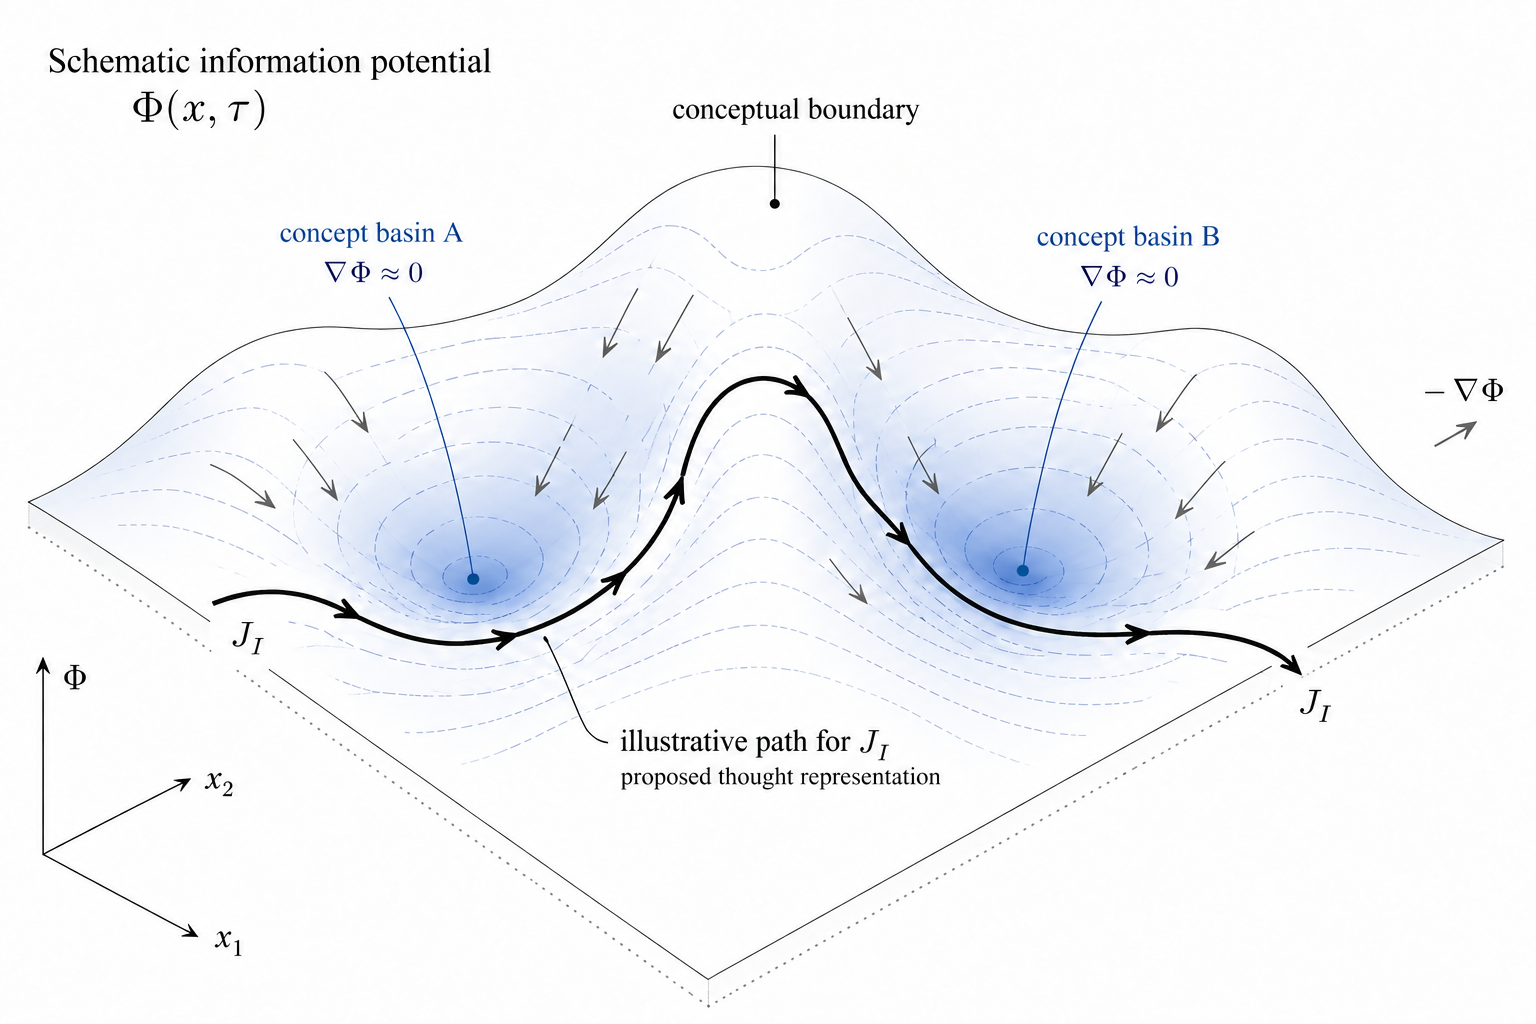
\includegraphics[width=0.92\linewidth]{figures/fig1_potential_geometry.png}
\caption{
情報ポテンシャルの幾何としての概念地形の模式図。
曲面はモデルのポテンシャル$\Phi(x,\tau)$を例示する。
盆地は$\nabla\Phi \approx 0$となる局所的な概念の定義を描く。
描かれた経路は流れ場$J_I$に関連づけた例示的な表現であり、場そのものでも、測定された思考経路でもない。
認知的な読みは提案であり、尾根はモデルレベルの概念境界を例示する。
}
\label{fig:potential-geometry}
\end{figure}

地形は、情報流$\JI$に関連する履歴形成的な幾何として、情報ポテンシャル$\Phi(x,\tau)$をモデル内で読むものである。
移動は$\JI$に関連する軌道表現であり、$-\nabla\Phi$は方向的な偏りを与えるが、経路全体を指定しない。
この移動を思考と呼ぶことは、さらに認知的解釈を加えることであって、場・経路・内容の同一性を意味しない。
理解の描像では、以前は困難だった領域での$|\nabla\Phi|$の局所的な減少を用いる。
感じられる容易さとの対応は仮説に留まる。形式的な閾値定義は、理解した感覚の独立した証拠ではない。

\subsection{谷としての概念}
この描像では、概念はポテンシャル地形の谷である。
それは$\Phi$が低く、軌道が自然に引き寄せられる領域である。
谷の深さには反復的な通過が反映されると提案し、幅はその概念が適用される文脈の広がりと比較する。
これらの比較は、独立した意味の測定を与えるものではない。

重要なのは、谷の中に意味が入っているわけではないという点である。
谷を\emph{動的アトラクタ}、すなわちモデル内で後続の軌道に偏りを与える領域として記述し、思考のパターンをその認知的解釈として提案する。
この枠組みで概念の「意味」と呼ぶものは、アトラクタが利用可能にする軌道の集合である。

\subsection{地形を形づくる操作としての言語トークン}
言語トークンは、自然言語の単語だけでなく、局所的な摂動として場に作用しうる、離散的で再アドレス可能なあらゆる媒体を含む広い意味で用いる。
記号、紋章、身振り、図、数式表記などが含まれる。
この記述では、それらに内在的な意味を割り当てない。
地形に偏りを与える局所的な摂動としてモデル化する。
類似した文脈での反復使用は、関連する谷を深めると仮定し、再利用の減少は浅化と関連づける。
送り手と受け手の地形がより似ていれば、摂動への反応もより似たものになりやすいと提案する。
地形の乖離は、コミュニケーションの失敗に寄与する可能性がある。
この比較仮説は、コミュニケーションの説明を尽くすものでも、コミュニケーションの成功から幾何を推定するものでもない。

\subsection{見えないGPU}
見えないGPUという比喩は、地形を直接調べることなしに認知を構造的に解釈する提案である。
思考が自然に浮かぶこと、つながりが自ずと示唆されること、理解が段階的に組み立てられるのではなく突然訪れること、といった経験例の整理に用いる。

これらの経験には、幾何の中に保存された内在的な意味ではなく、$\Phi$の幾何との対応を提案する。
これは主観的経験がどのように生成されるかの説明ではない。

以下の節では、この直観的語彙を形式的定義、および未解決の認知的・現象的対応写像から区別する。
